%=== CHAPTER FIVE (5) ===
%=== Discussion ===

\chapter{Result \& Discussion}
\begin{spacing}{1.5}
\setlength{\parskip}{0.3in}
\begin{figure}[h]
    \centering
    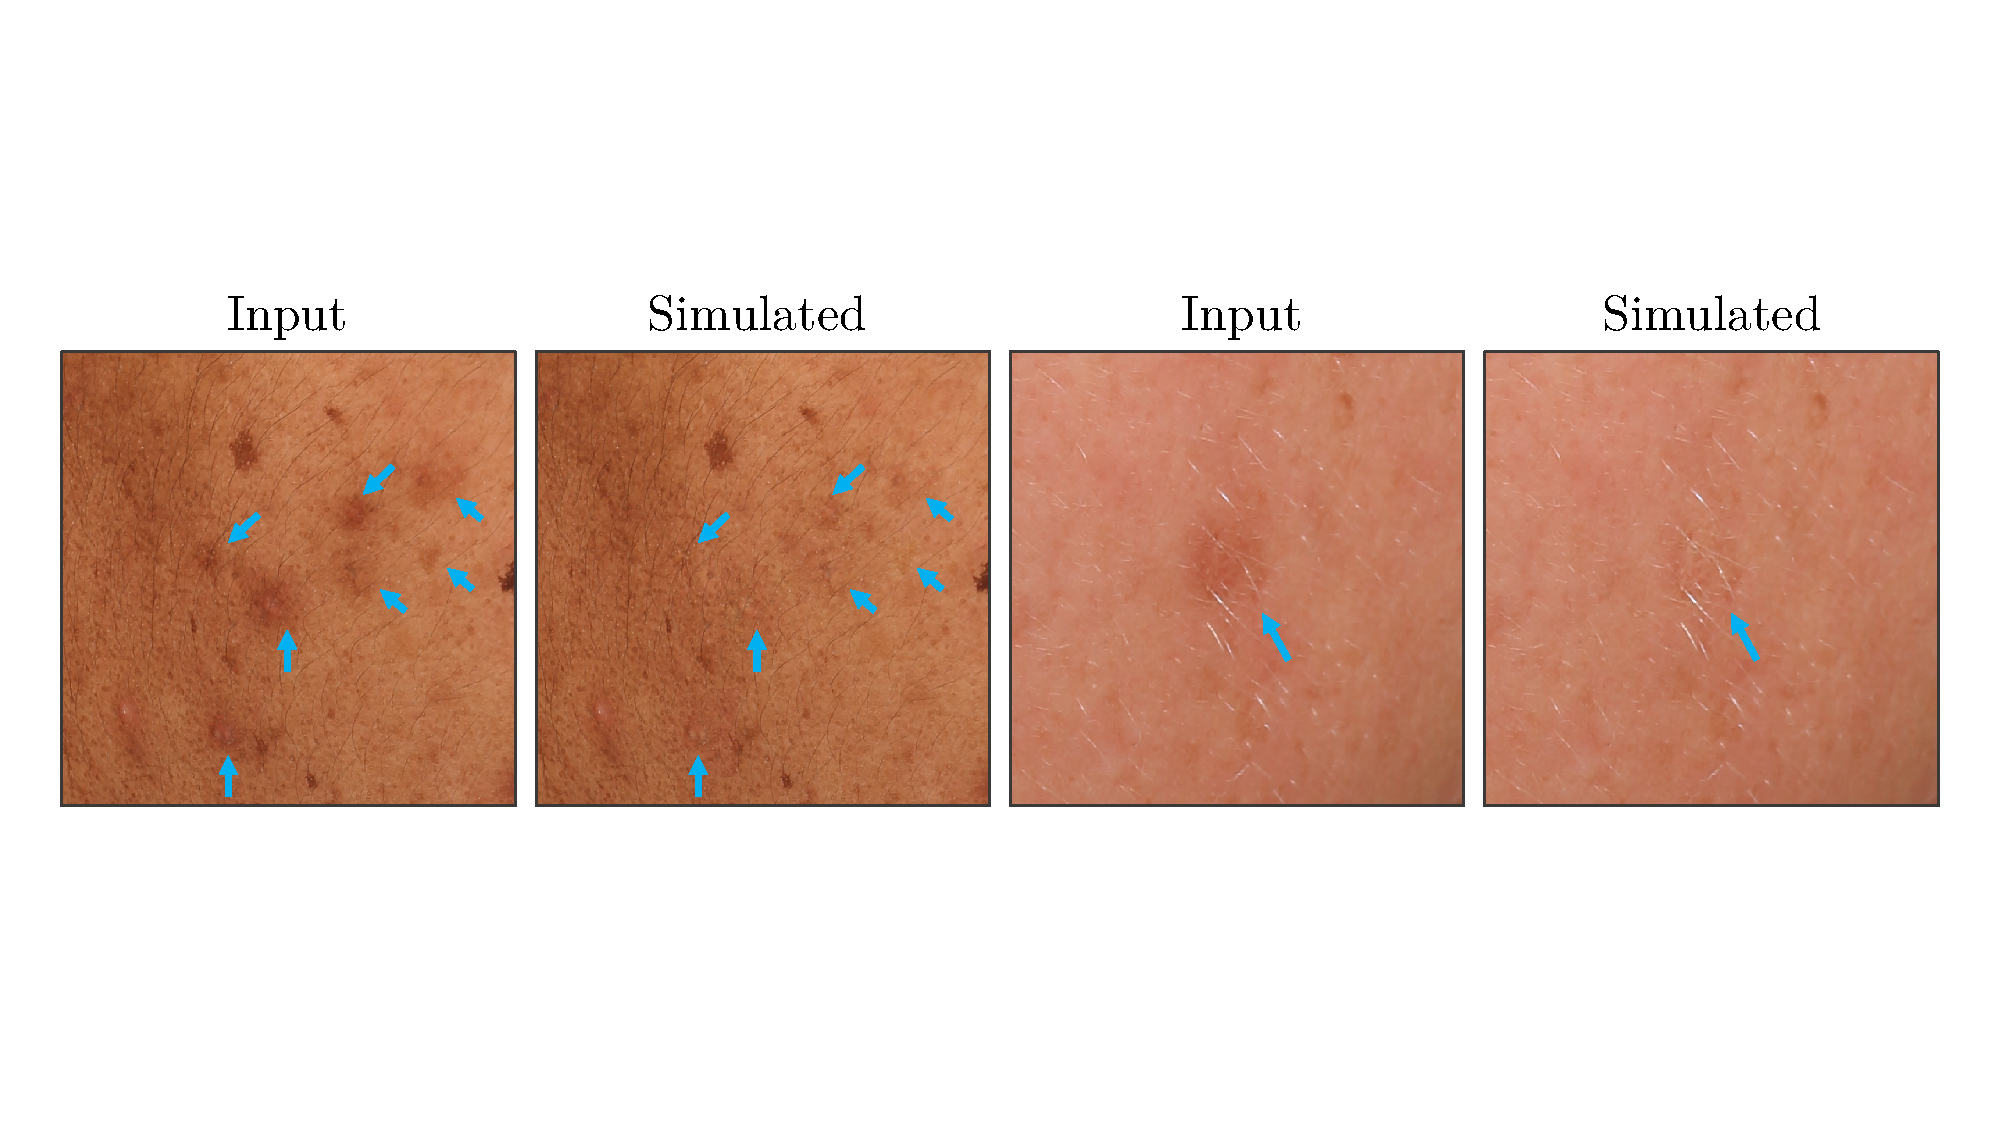
\includegraphics[width=0.9\linewidth]{Chapter5/img_comp2.pdf}
    \caption{Zoomed-in detail of the blemish fading simulation results. Blue Arrows are manually added to highlight blemishes of interest (acne or pigmentation). Note that our method can keep skin details (e.g. hairs, texture) unaltered.}
    \label{fig:sim2}
\end{figure}
We evaluate simulation quality and result in terms of versatility, reality, and controllability. A detailed discussion of each aspect follows.

\section{Versatility}
Versatility is a key attribute of the algorithm's ability to be generalized to various scenarios. By testing various patterns and degrees of pigmentation, acne, and other skin aberrations, we demonstrated the successful application of the algorithm on multiple skin tones and different types of skin blemishes. Figure \ref{fig:sim1} clearly illustrates how the algorithm accurately models the local chromophore enrichment of the skin, thus realizing genuine blemish change simulation. Particularly noteworthy is that our method maintains the subtle textures of the skin unaltered, such as fine hairs or pores are shown in Figure \ref{fig:sim2}, further proving its high precision and usability.
\begin{figure}[t]
    \centering
    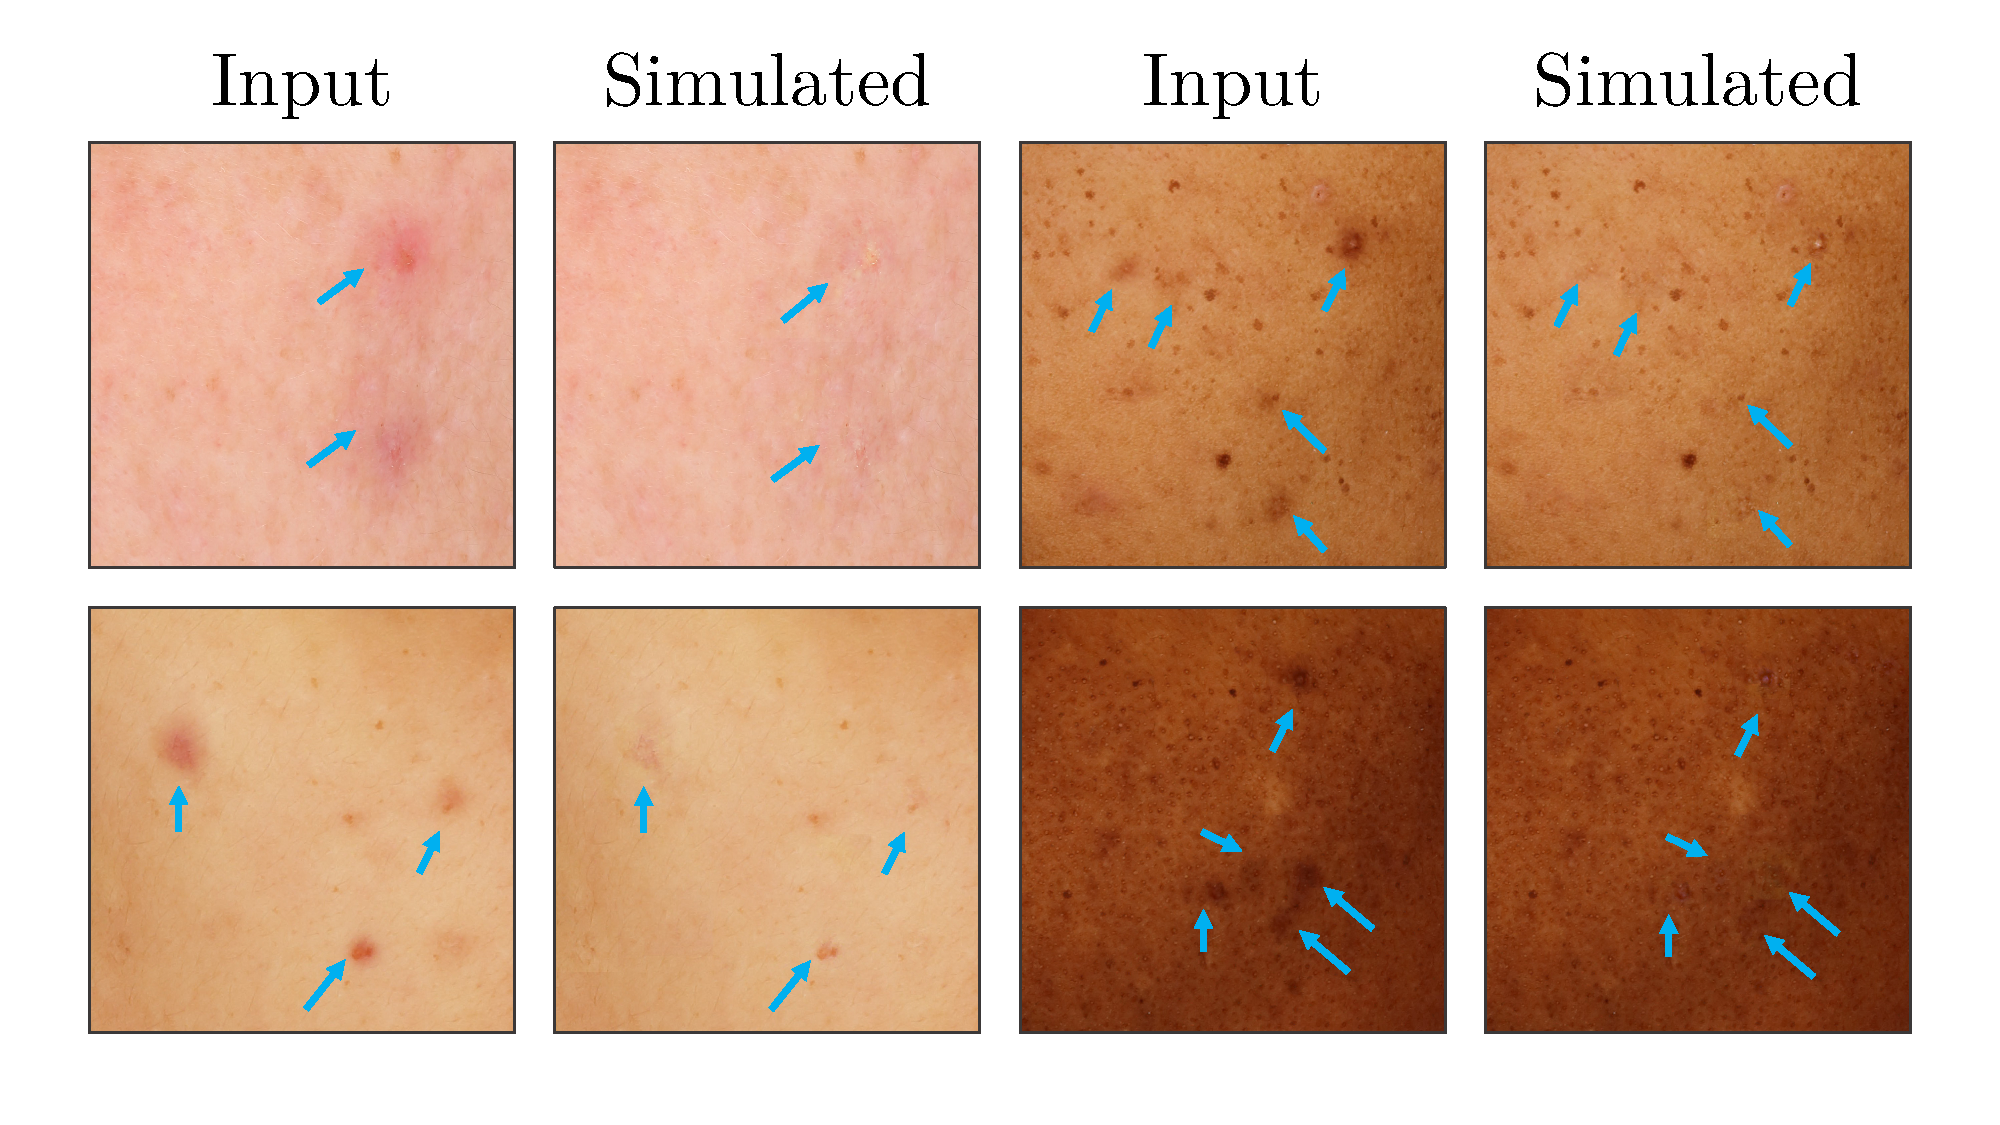
\includegraphics[width=\columnwidth]{Chapter5/img_comp4.pdf}
    \caption{Simulation under various skin tones}
    \label{fig:sim1}
\end{figure}

\section{Reality}
\begin{figure}[t!]
    \centering
    % \begin{subfigure}
    %     \centering
        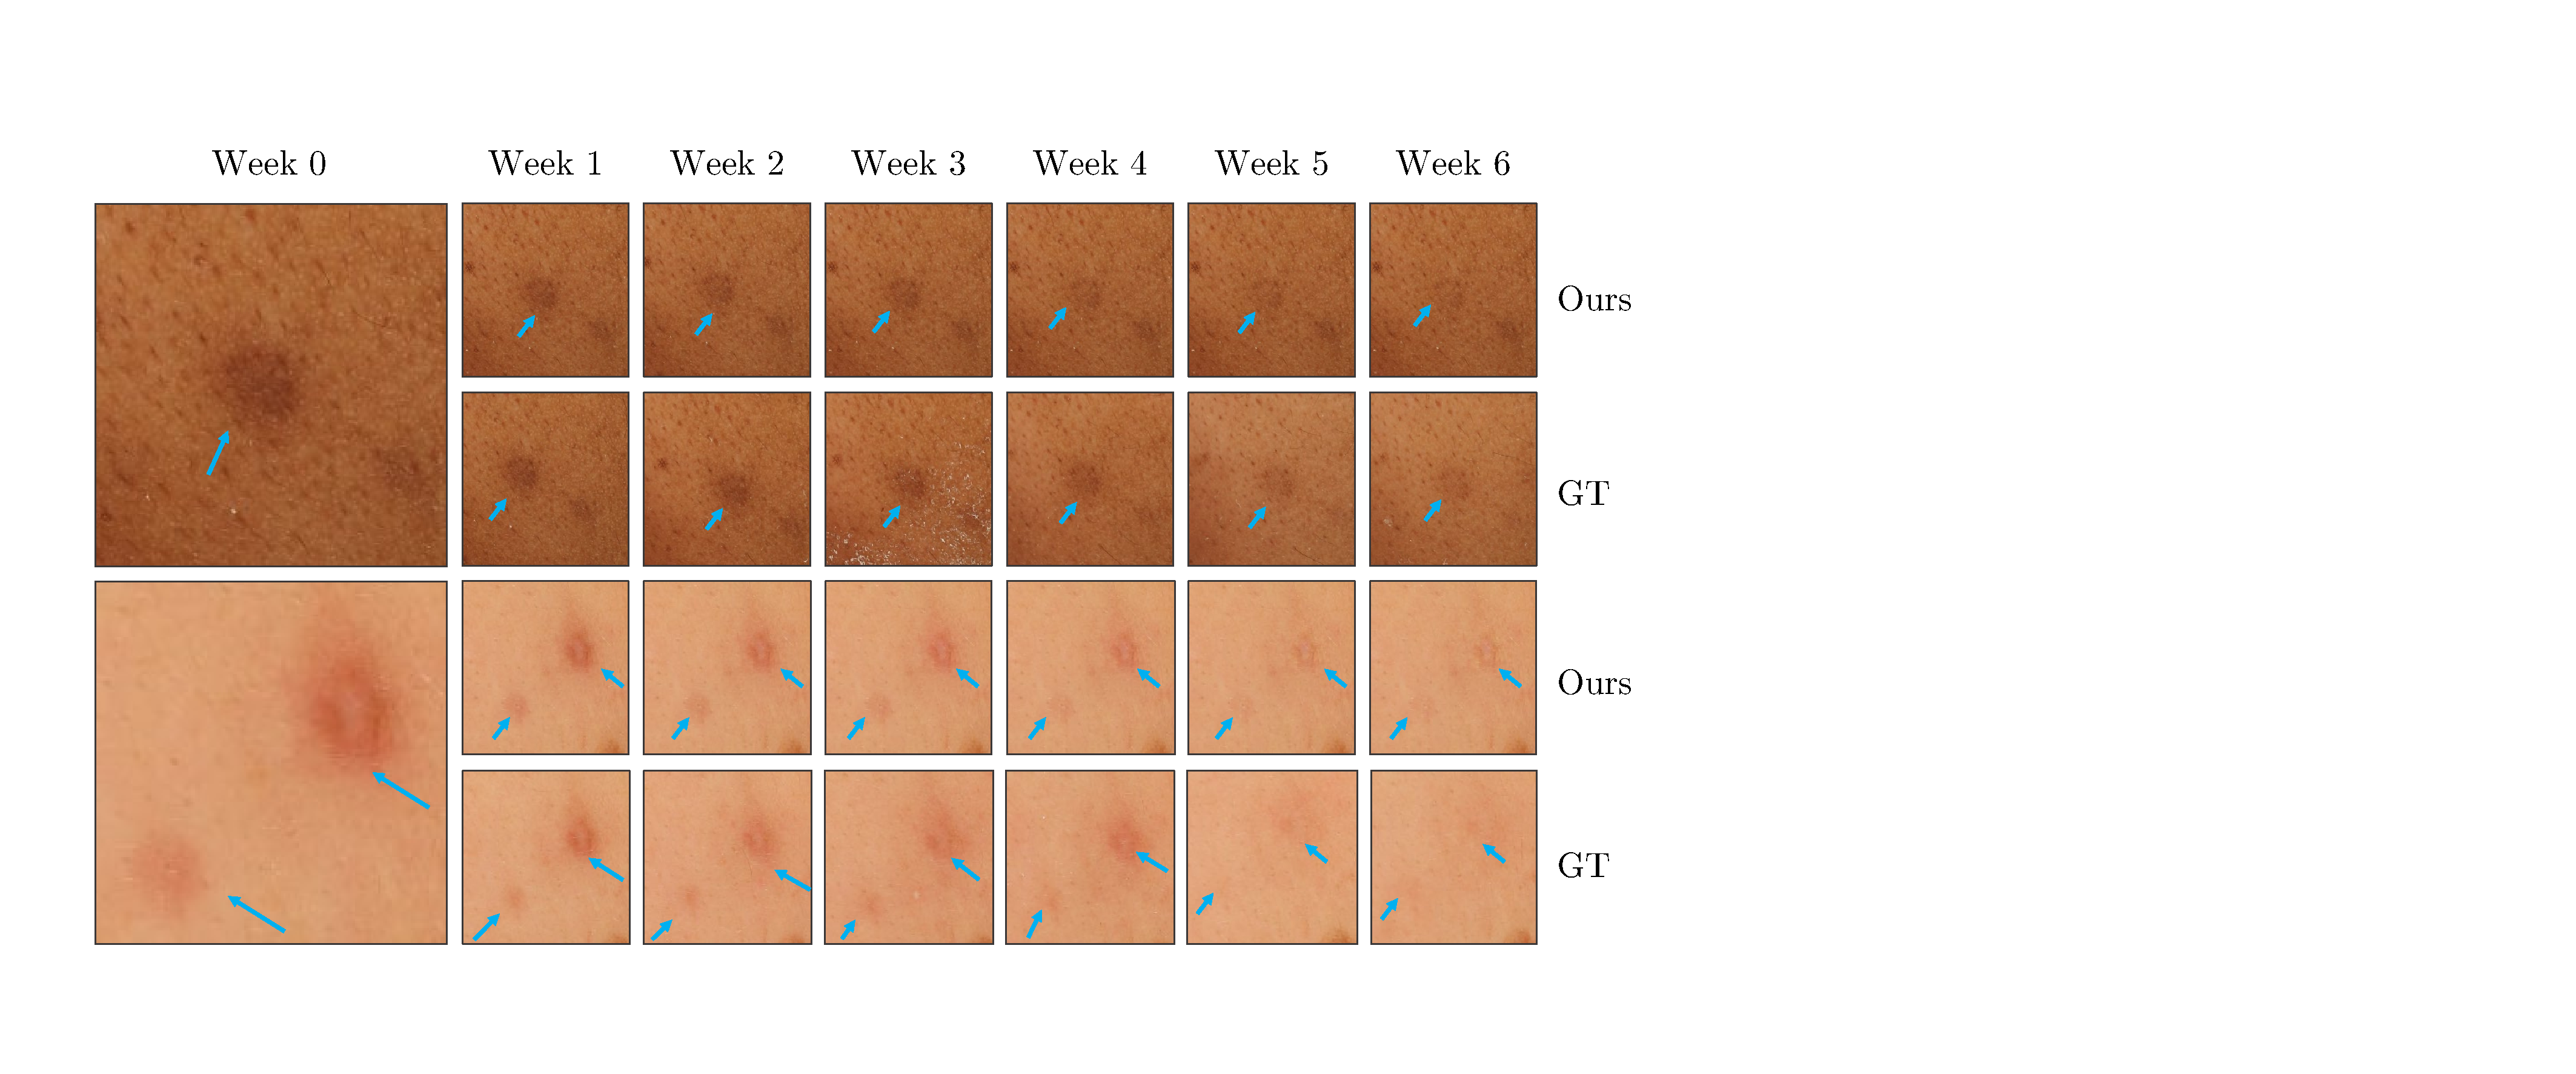
\includegraphics[width=\columnwidth]{Chapter5/forward3.pdf}
        \caption{Simulation of blemish fading process}
    % \end{subfigure}
    % \vspace{2em}

    \caption{We show the application of our method to the simulation of the fading process of skin blemish. Blue Arrows are manually added to highlight blemishes of interest (acne or pigmentation). In our simulation, we input images of \textit{Week 0} and adjust the parameters of the obtained model to simulate the change of the blemishes in the following weeks. Note that our method applies to different skin tones and various types of blemishes.}
    \label{fig:forward}
\end{figure}
Exploration of reality evaluates the algorithm's ability to simulate complex changes in real human skin conditions. We first selected some skin blemish samples with long-term evolution patterns from the dataset and simulated them using our algorithm. Figure \ref{fig:forward} shows one example, revealing the gradual fading of pigmentations over 7 weeks. Our algorithm successfully simulates the natural fading trajectory of the pigmentations, showing a natural change in color.

For the PS method, we utilized the inpainting tool of the software, selecting and removing blemishes on the original image under the Content-Aware mode. The modified image was then combined with the original image through Alpha blending. For the SD method, we used the inpainting mode and set the text prompt as \texttt{skin patch, human face skin, high definition, best quality}. Each test was performed with 50 iterations of sampling using the \texttt{DPM++SDE Karras} sampler, with the random seed fixed to 42. We adjusted the denoising ratio to increase the difference between the generated image and the original.

We calculated Fréchet Inception Distance (FID) scores for the simulated images and the ground-truth images to quantitatively measure the quality of algorithms for skin blemish editing. The results are displayed in Table \ref{tbl:fid} and the visual comparison is shown in Figure \ref{fig:baseline}.
\begin{figure}[t!]
    \centering
    \begin{subfigure}{.9\textwidth}
        \centering
        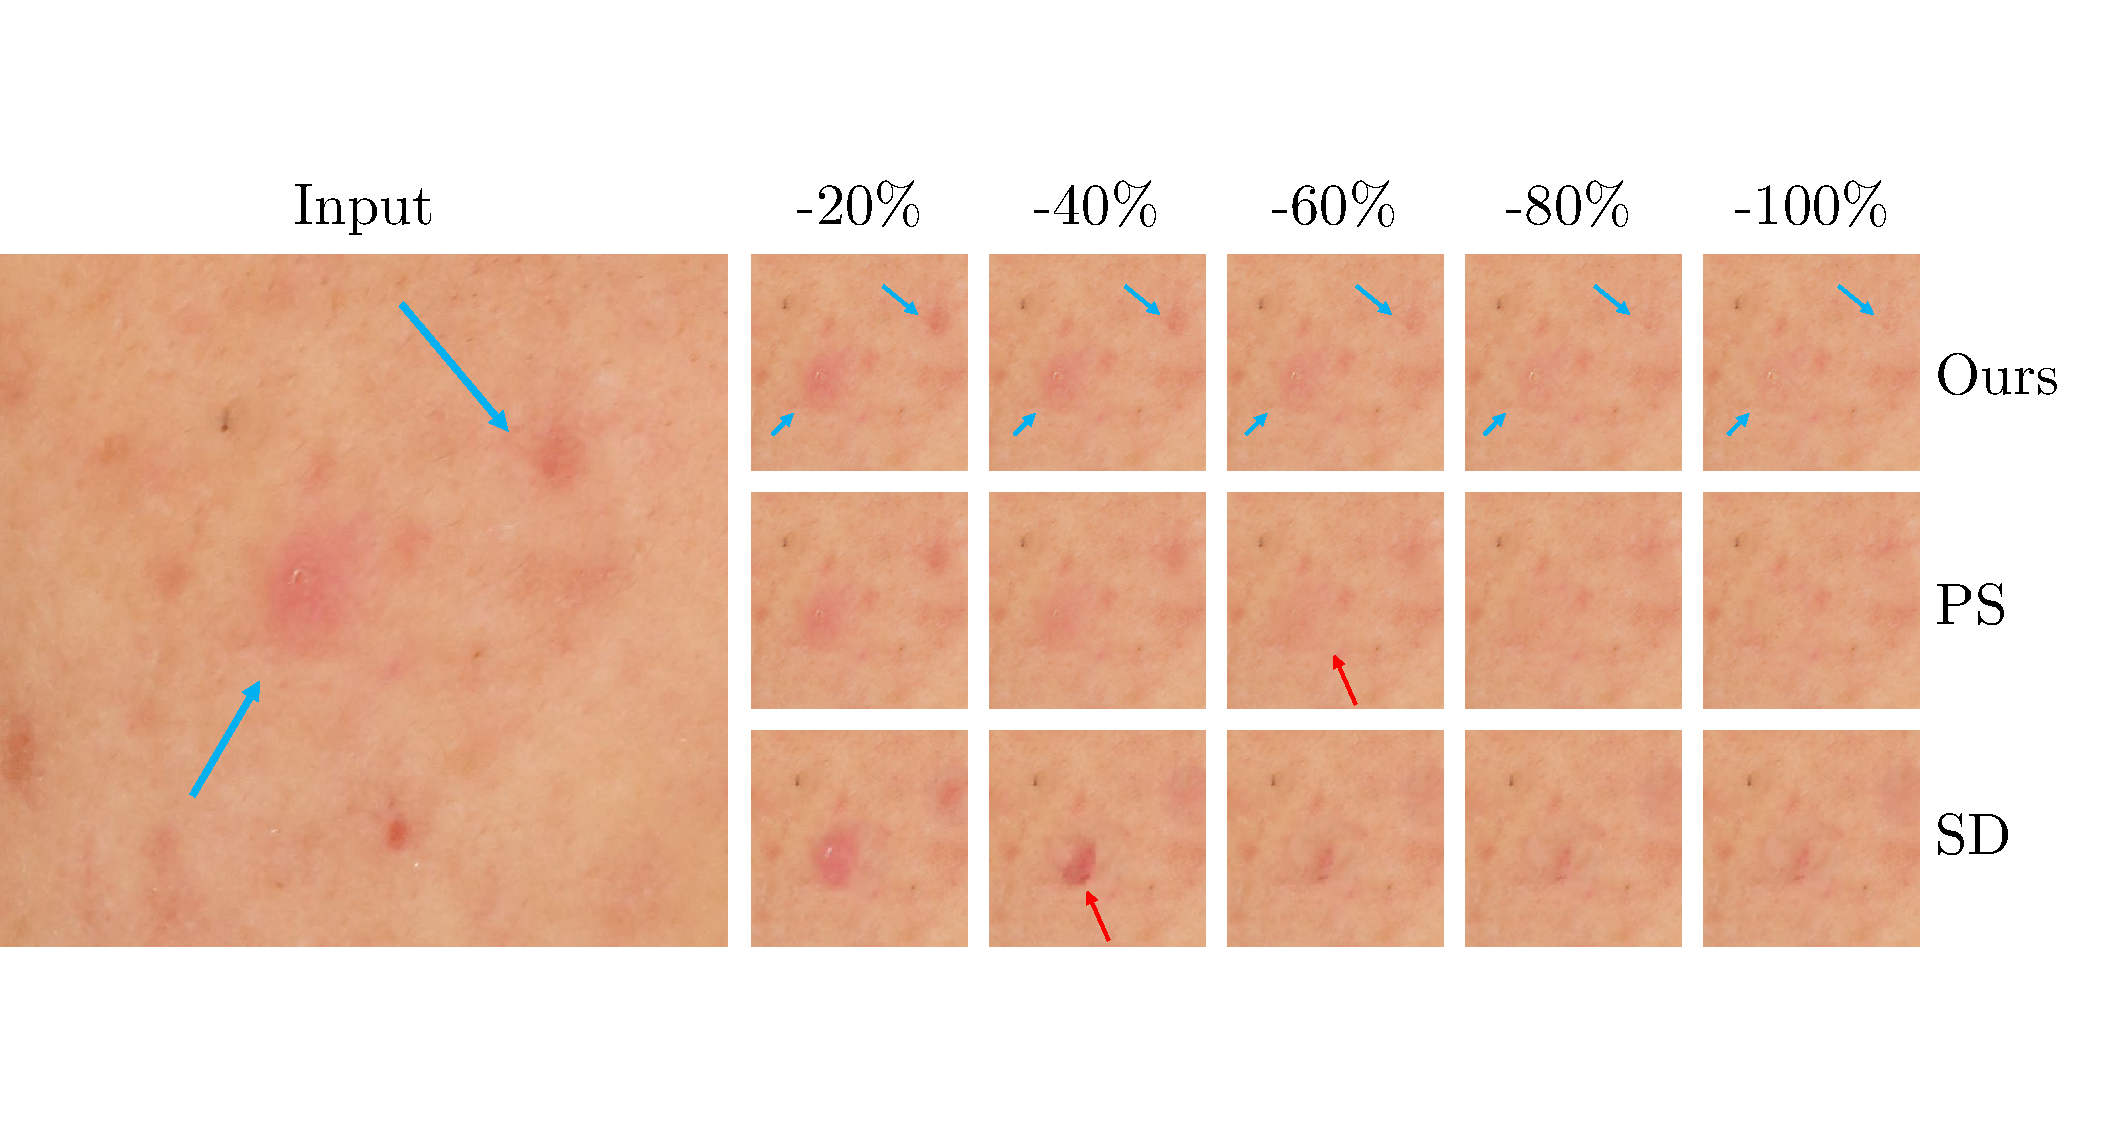
\includegraphics[width=\linewidth]{Chapter5/baseline11.pdf}
    \end{subfigure}
    \hfill
    \begin{subfigure}{.9\textwidth}
        \centering
        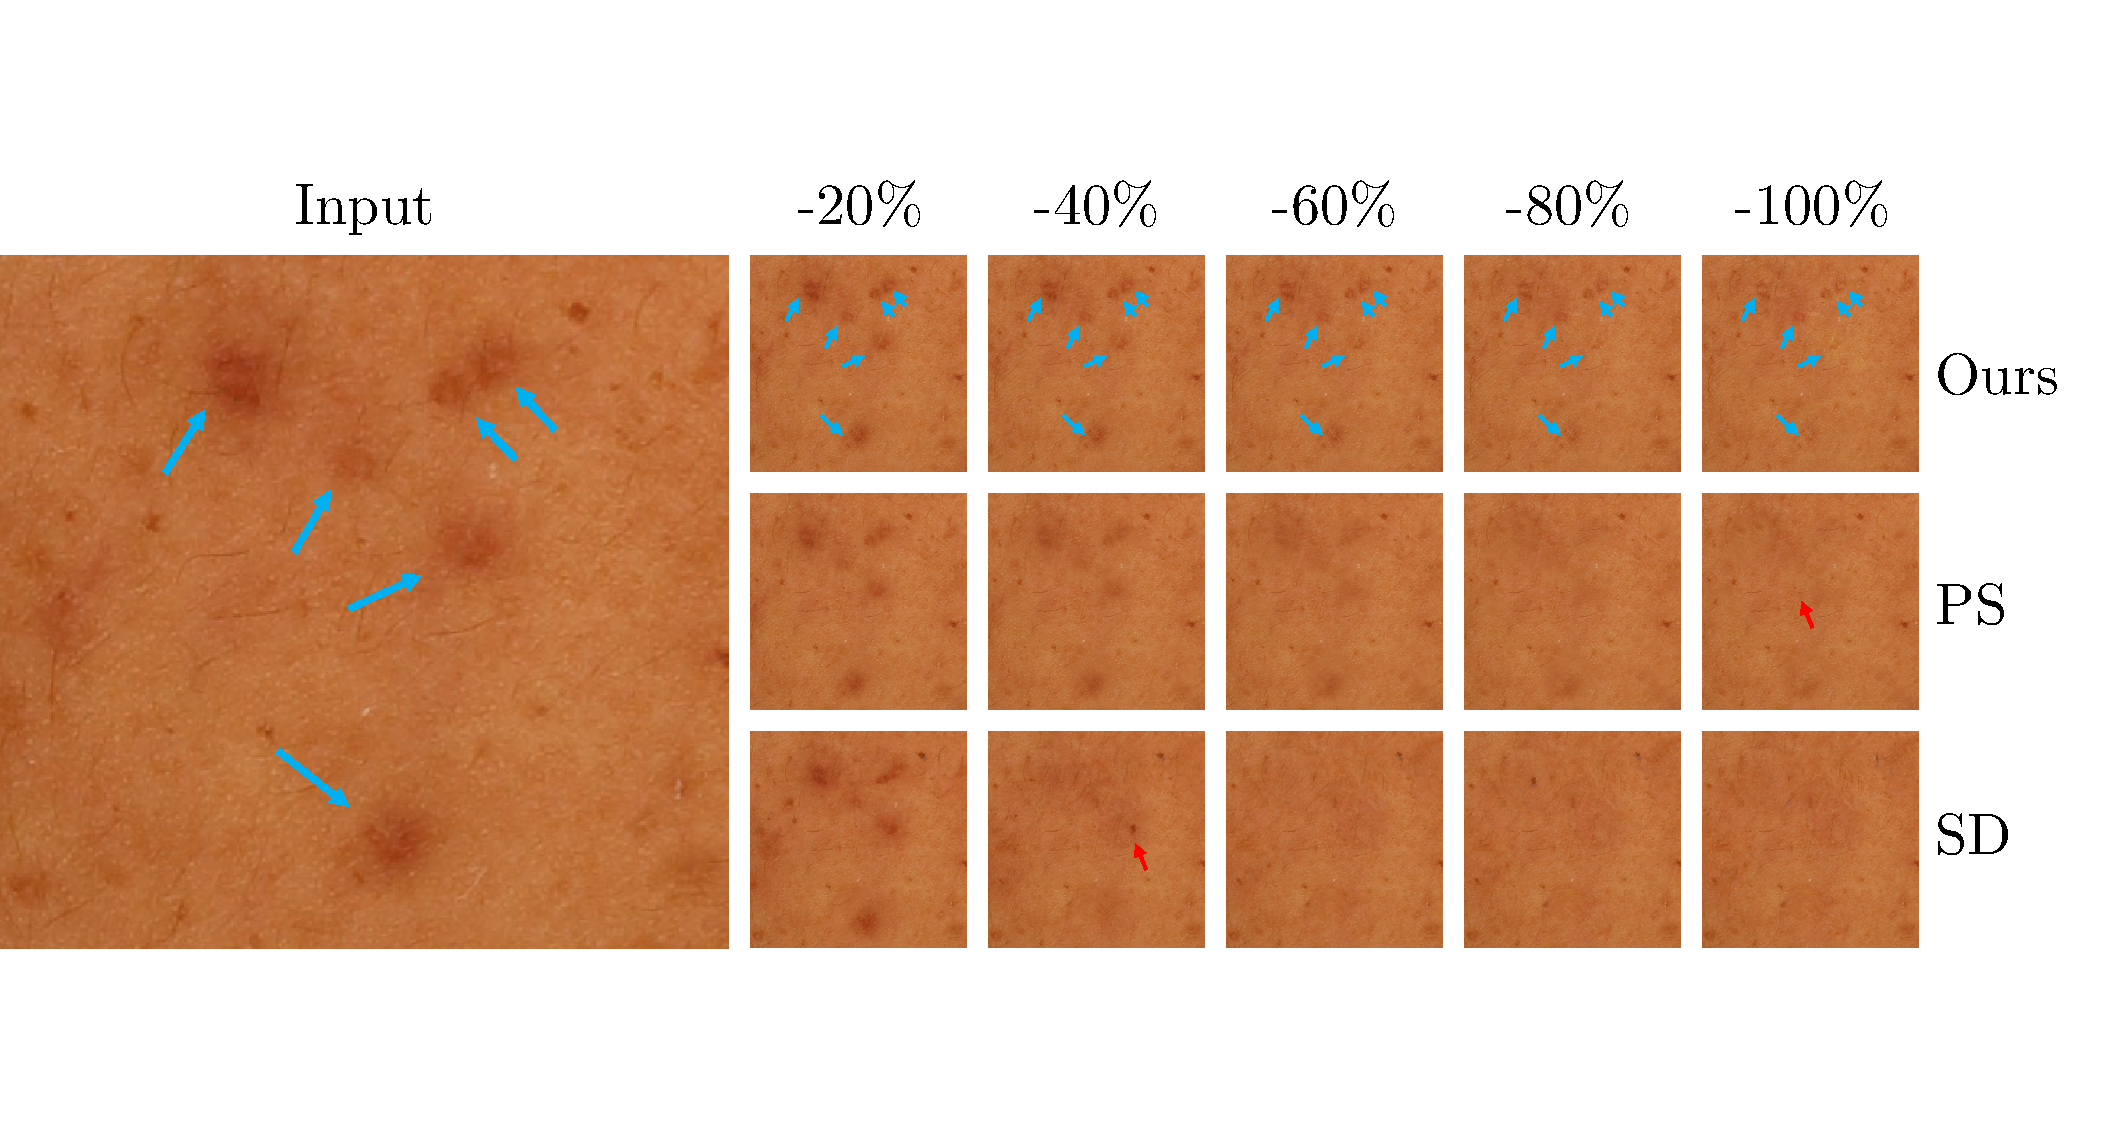
\includegraphics[width=\linewidth]{Chapter5/baseline12.pdf}
    \end{subfigure}
    \caption{Comparison with baseline methods. We compared the results of several blemish removal or modification methods, including our method (marked as Ours), Adobe Photoshop\cite{adobephotoshop} inpainting (marked as PS), and Stable Diffusion\cite{rombach2021highresolution} inpainting (marked as SD). Arrows are manually added to highlight areas of interest. Note the red arrows where the PS produces over-smoothed skin patches and the SD produces visible artifacts.}
    \label{fig:baseline}
\end{figure}

\begin{table}[t!]
    \caption{FID scores of different blemish fading rates. Lower scores are better.}
    \resizebox{\columnwidth}{!}{%
        \begin{tabular}{cccccc}
            \hline
            \multirow{2}{*}{Methods} & \multicolumn{5}{c}{Fading Rate}                                                                         \\ \cline{2-6}
                                     & 100\%                           & 80\%            & 60\%            & 40\%            & 20\%            \\ \hline\hline
            SD                       & 144.89                          & 133.53          & 134.16          & 160.10          & 159.54          \\
            PS                       & 117.98                          & 120.37          & 125.15          & 129.26          & \textbf{129.96} \\
            \textbf{Ours}            & \textbf{115.30}                 & \textbf{118.12} & \textbf{122.64} & \textbf{127.09} & 131.60          \\ \hline
        \end{tabular}%
    }
    \label{tbl:fid}
\end{table}

For the FID scores, our method achieved the lowest scores in the vast majority of cases, except for the 20\% fading rate. In particular, our proposed method has less variation in FID scores compared to other baselines at different fading Rates, which suggests that our model is able to achieve robust, realistic skin blemish simulations.

Visual comparison more intuitively demonstrates the superiority of our algorithm. The PS method, although straightforward, led to a loss of skin detail through simple interpolation, resulting in blurry patches. On the other hand, the SD method was able to generate some contextually coherent skin details while removing the blemishes, but its quality was limited. Specifically, at higher denoising ratios, the SD method produced noticeable artifacts, and the modified areas differed in color from the surrounding skin.

Our method not only closely aligns with the natural degradation process of real skin, but also ensures that the modified pigmentations match the underlying skin seamlessly. Unlike other techniques, our approach does not create artifacts or blurriness. It maintains skin details, including subtle textures such as hair and pores, leading to a natural appearance. This underlines the effectiveness of our method in preserving the intricacy of skin texture while accomplishing realistic modifications.

\begin{figure}[t!]
    \centering
    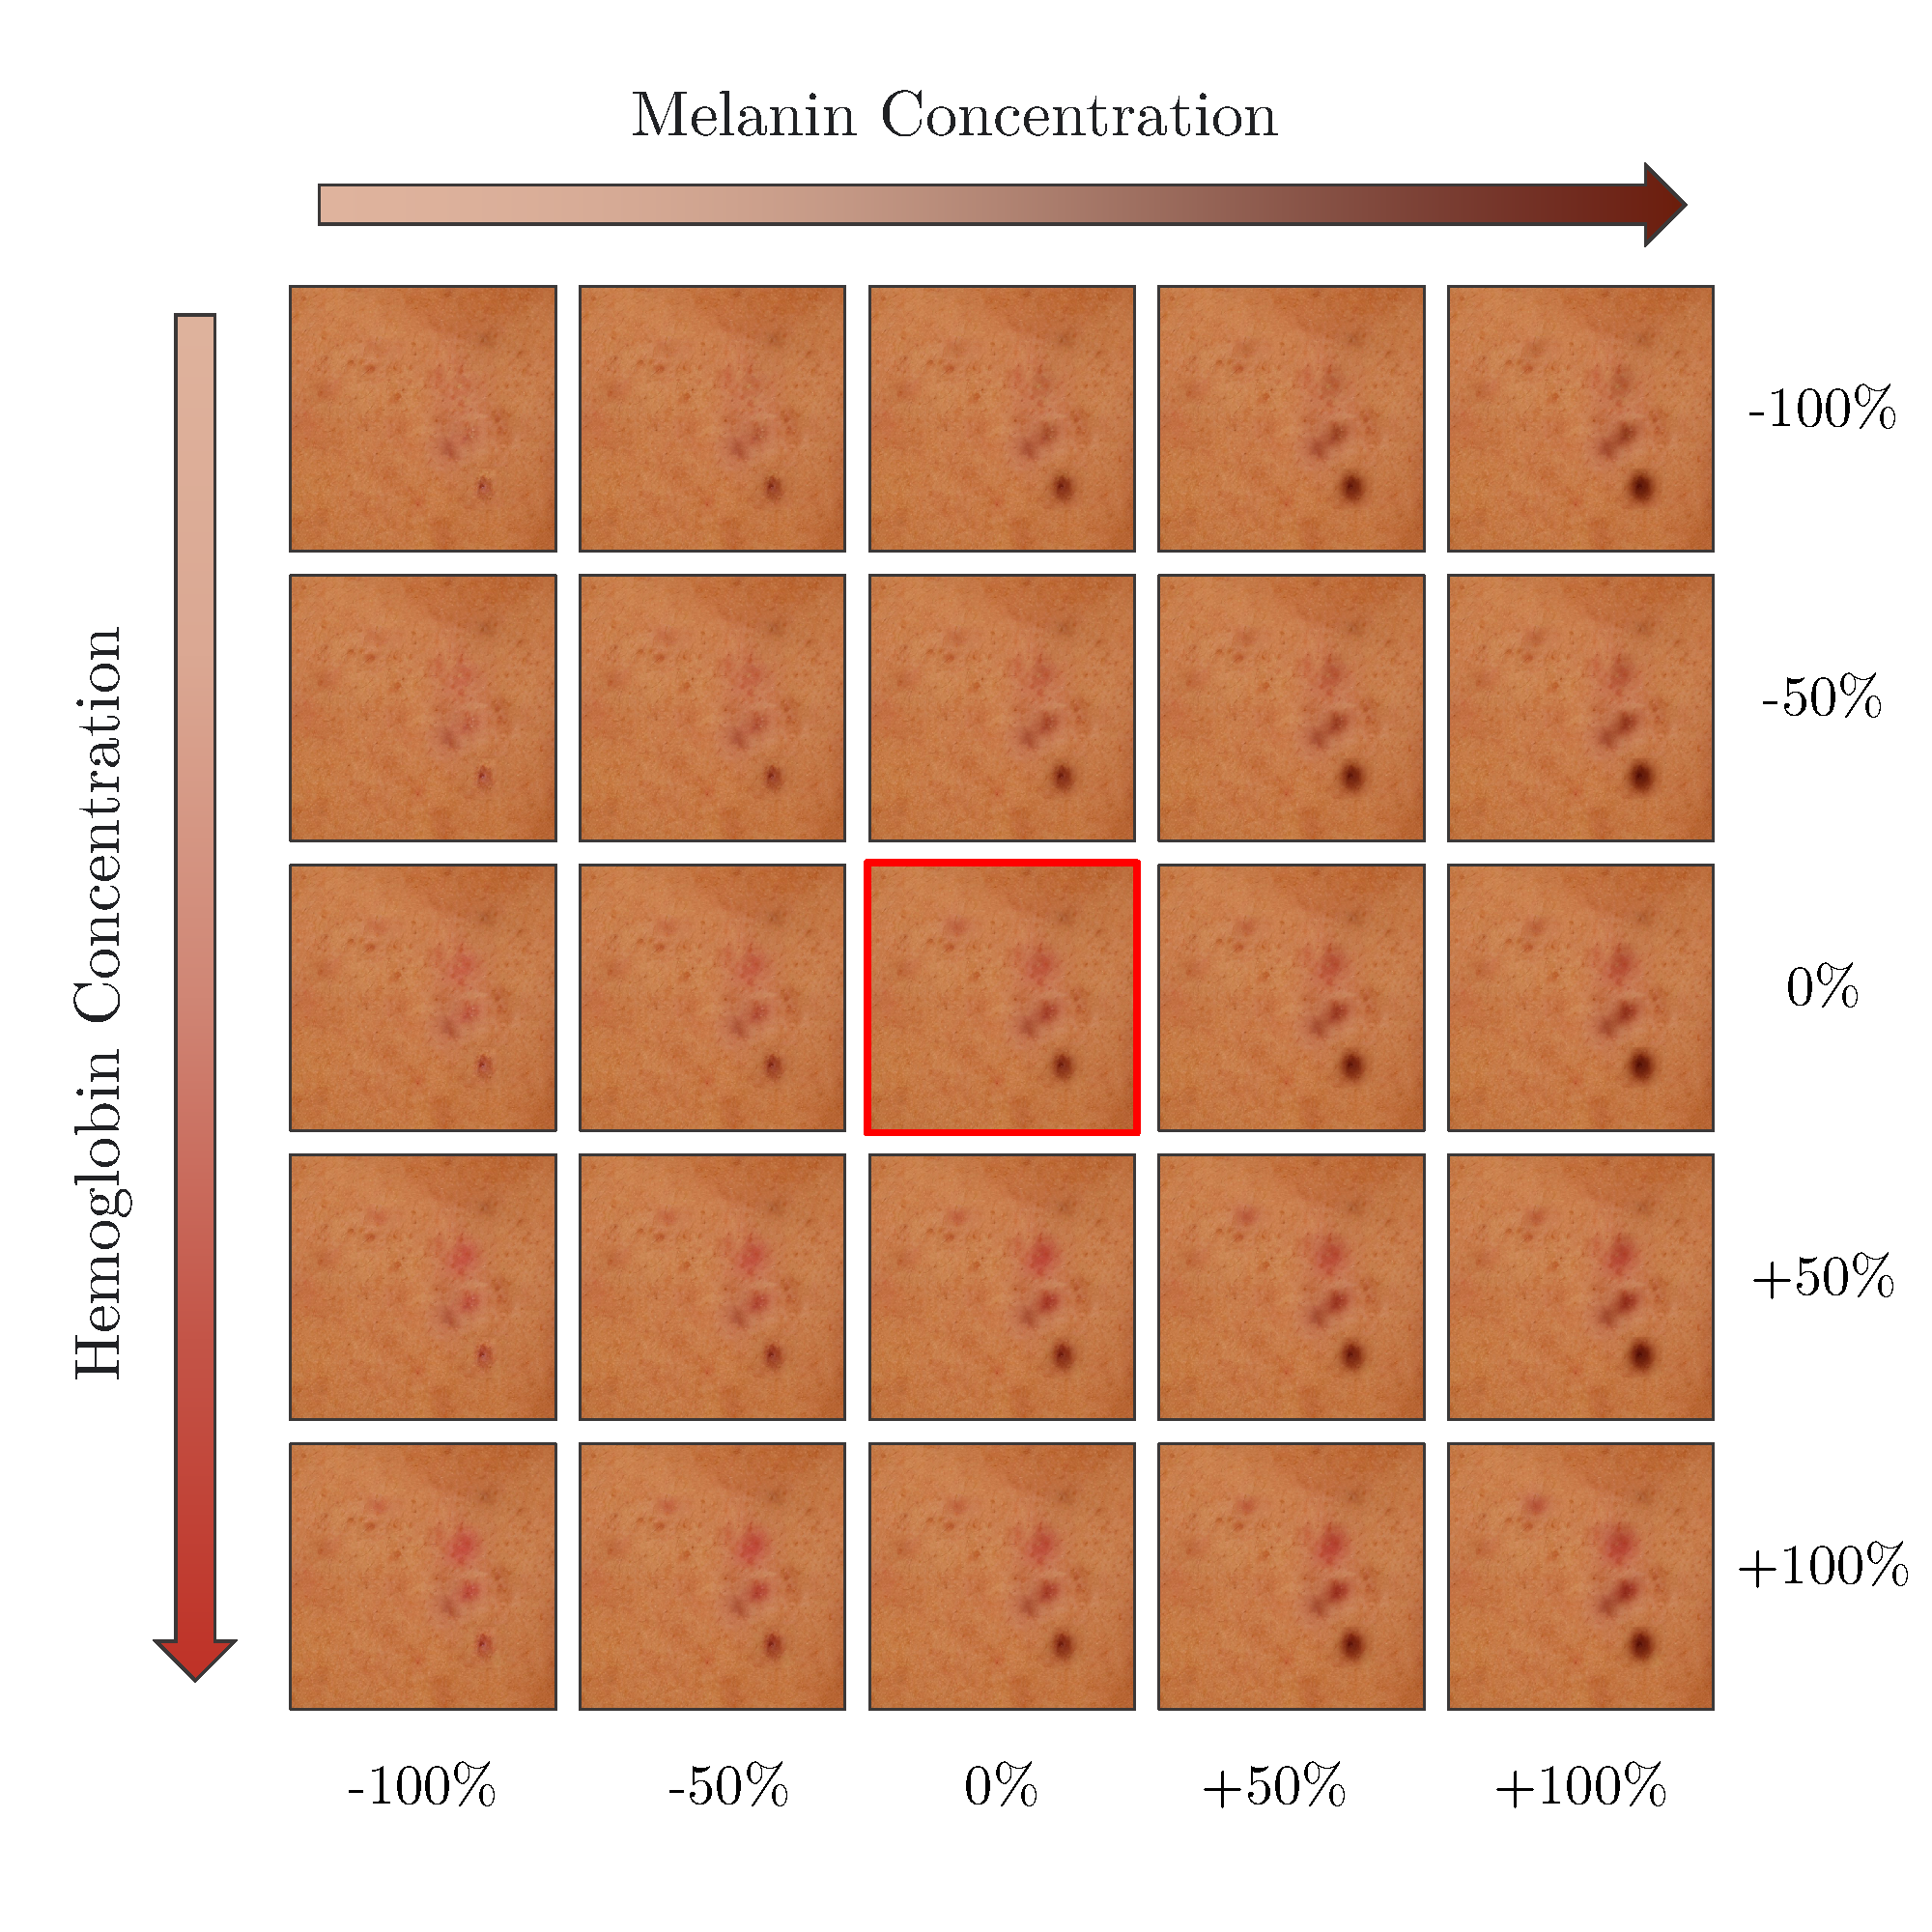
\includegraphics[width=0.96\columnwidth]{Chapter5/grid.pdf}
    \caption{Matrix of different chromophore concentrations setting. The original image is marked by a red box. Our model fully decouples the major chromophores of human skin, enabling highly controllable pigmentation editing.}
    \label{fig:matrix}
\end{figure}

\section{Controllability}
Controllability is a key to user interaction with the algorithm. One significant advantage of our model is its high controllability, where users can freely adjust the parameters of the pigmentation to precisely control its appearance.
We plotted a changing matrix by adjusting the concentration control parameters of melanin and heamoglobin, shown in Figure \ref{fig:matrix}. Our method successfully decouples the concentrations of these two chromophores, allowing users to independently control their apparent features, thus flexibly simulating the change of blemishes under different conditions.

\section{Perception Study}
\begin{figure}[t!]
    \centering
    \begin{subfigure}{.9\textwidth}
        \centering
        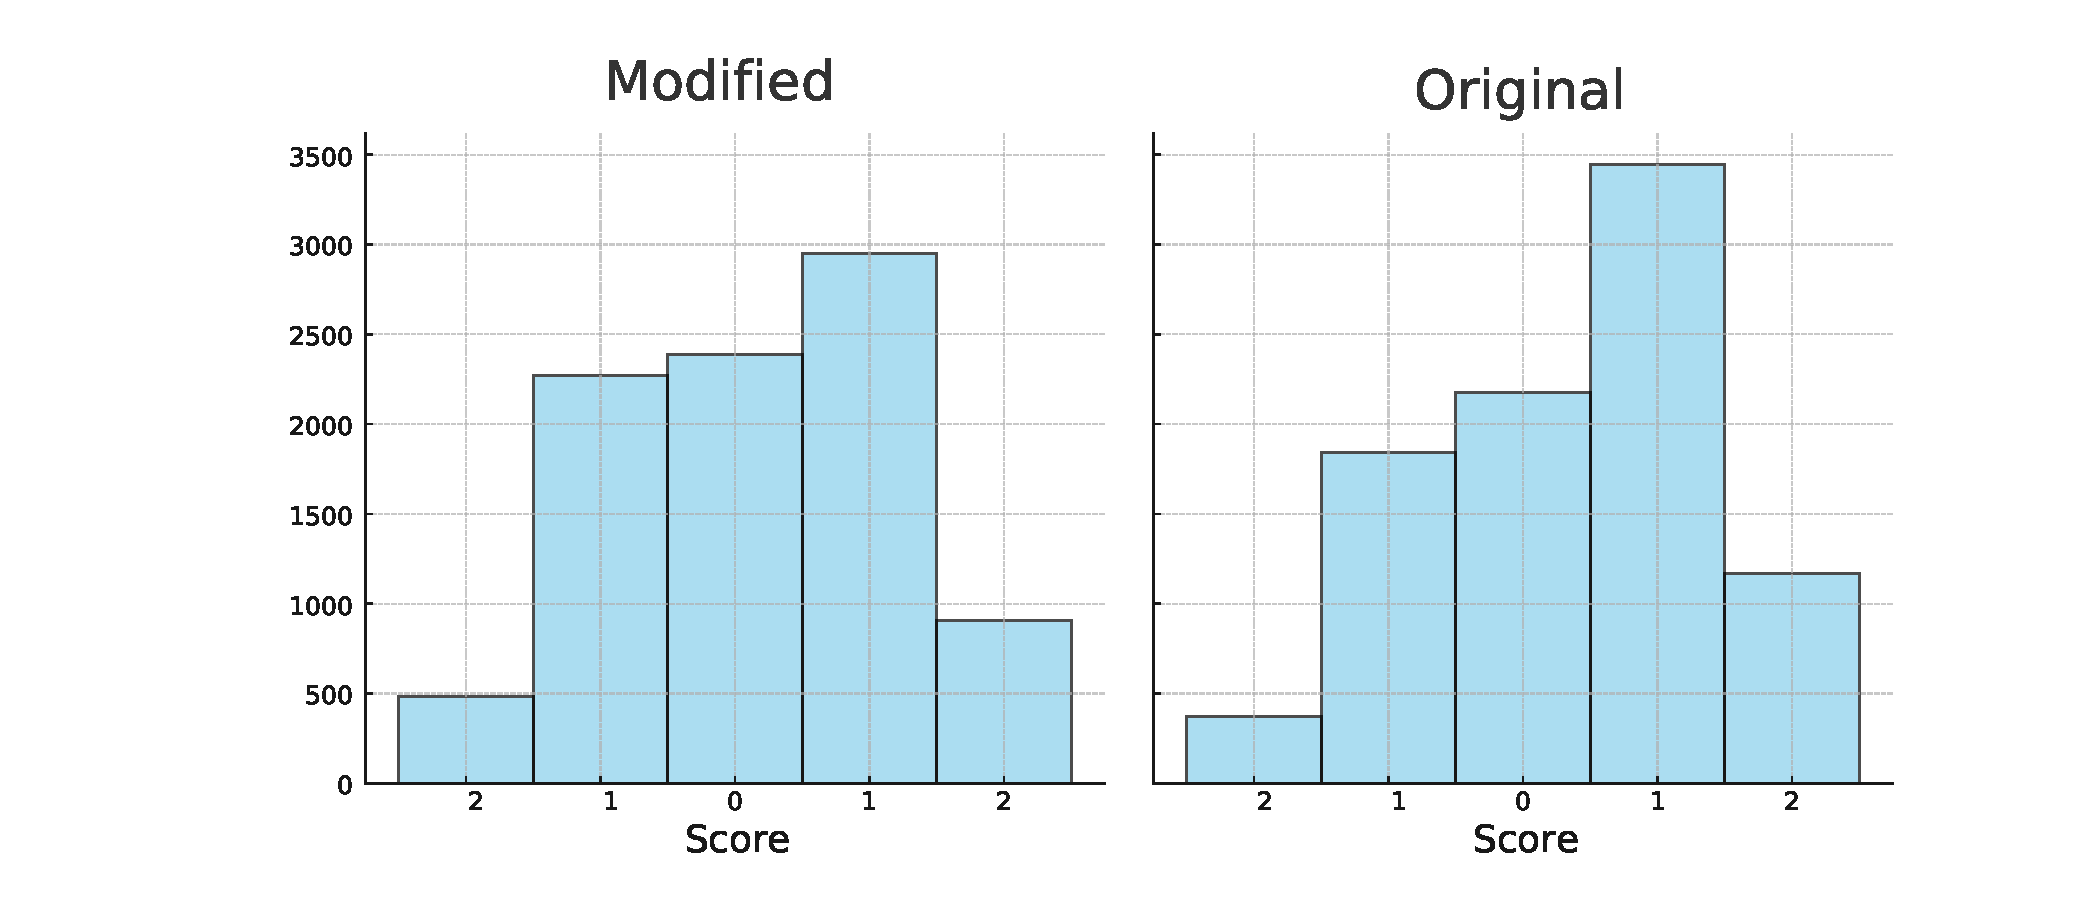
\includegraphics[width=0.95\columnwidth]{Chapter5/score.pdf}
        \caption{Scoring frequencies of survey responses}
        \label{fig:survey_hist}
    \end{subfigure}\hfill
    \begin{subfigure}{.9\textwidth}
        \centering
        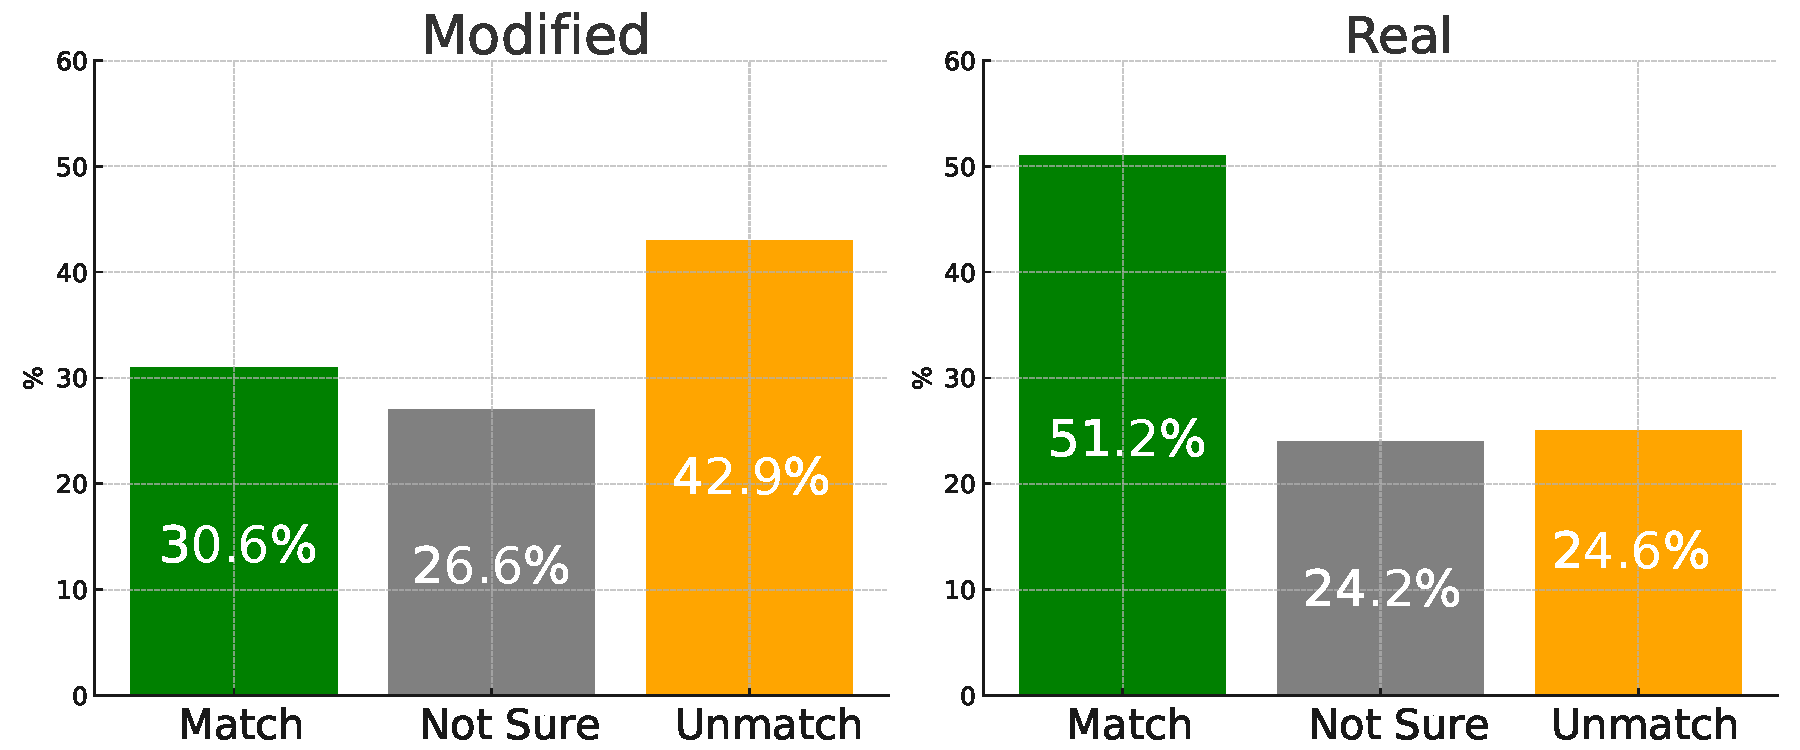
\includegraphics[width=0.95\columnwidth]{Chapter5/bar_charts_modified.pdf}
        \caption{Bar chart of survey results}
        \label{fig:bar_charts}
    \end{subfigure}
    \caption{Panellists scored images from -2 to +2 to assess their confidence in considering the image as modified or not, with higher scores indicating that the user considered the image to be unmodified. Scoring frequencies are displayed in Figure \ref{fig:survey_hist}. The results of the survey are shown in Figure \ref{fig:bar_charts}. For the modified images, more people perceived them as unmodified or not sure. This suggests that our modifications are consistent with human perception and intuition.}
\end{figure}
The objective of this study was to evaluate if the pigmentation simulation was natural and believable. In the test, as shown in Figure \ref{fig:bar_charts}, the altered images had a lower average score (0.16956 vs 0.35511), only 30.6\% correctly identifying the altered image vs 23.6\% judging the real images as altered, and 26.6\% not sure if it is or is not altered. This indicates that the effect of our proposed algorithm is superior, to the point where laypeople cannot readily discern traces of algorithmic alteration.

%=== END OF CHAPTER FIVE ===
\end{spacing}
\newpage
